\documentclass[sigconf, anonymous]{acmart}

\settopmatter{printfolios=true}
\raggedbottom

\AtBeginDocument{%
  \providecommand\BibTeX{{Bib\TeX}}}

\setcopyright{acmlicensed}
\copyrightyear{2026}
\acmYear{2026}
\acmDOI{XXXXXXX.XXXXXXX}
\acmConference[ICAIF '26]{7th ACM International Conference on AI in Finance}{November 2026}{Milan, Italy}
\acmISBN{978-1-4503-XXXX-X/2026/11}

\usepackage{amsmath,amsfonts}
\usepackage{amsthm}
\usepackage{booktabs}
\usepackage{graphicx}
\usepackage{xcolor}
\usepackage{enumitem}
\usepackage{algorithm}
\usepackage{algorithmic}

\newtheorem{definition}{Definition}

\title{Predicting Decision-Time Reliability of Equity Market Risk under Delayed Inputs and Non-Stationary Conditions}

\author{Medha Kumar}
\affiliation{%
  \institution{National Institute of Technology Surat}
  \city{Surat}
  \state{Gujarat}
  \country{India}
}
\email{medha0214@gmail.com}

\begin{abstract}
Value-at-Risk (VaR) models are standard in automated risk control, yet
operational pipelines consume risk reports with a one-day reporting lag
while market regimes shift faster than the estimator adapts. This
mismatch creates a \emph{decision-time gap} in which a nominally
current risk estimate is stale. We formalise the \textbf{Decision-Time
Reliability} problem and propose a predictive monitoring layer that
estimates next-day failure probability using only decision-time
information. Leave-one-out ablation and SHAP analysis independently
confirm that risk-volatility divergence is the dominant predictive
signal---dominant by a $2\times$ margin in mean absolute SHAP
value---and that removing noisy features improves XGBoost ROC-AUC from
0.642 to 0.685. We compare four models across six global equity markets:
S\&P~500, FTSE~100, Nikkei~225, DAX, Hang~Seng, and EM ETF. A
reliability-gated three-level exposure policy reduces Expected Shortfall
Breach (ESB) by 49--69\% consistently across all six assets. Our novel
\textbf{Regime-Conditional Reliability Estimator} (RCRE) achieves the
best tail-severity reduction (50\% ESB reduction on S\&P~500) via soft
Gaussian regime mixing. The COVID-19 volatility shock, used as a fully
held-out stress test, confirms early warning capability during the acute
mid-March crash window.
\end{abstract}

\ccsdesc[500]{Computing methodologies~Machine learning}
\ccsdesc[300]{Applied computing~Economics}

\keywords{Value-at-Risk, reliability monitoring, regime detection, XGBoost, financial risk}

\begin{document}
\maketitle

%%─────────────────────────────────────────────────────────────
\section{Introduction}

Risk limits are enforced using model-derived signals that are rarely
synchronised with the market state at decision time. VaR models are a 
regulatory cornerstone of market risk practice~\cite{basel2019}, yet VaR 
and ES estimates are produced on rolling windows and published with delay, 
while volatility and tail behaviour can shift abruptly~\cite{cont2001empirical}.
Machine learning has demonstrated strong results in non-stationary financial 
settings~\cite{dixon2020machine}. We treat this as a \emph{systems problem}: 
rather than redesigning the base estimator, we learn a reliability monitor 
that predicts \emph{when} the reported risk will fail to bound next-day losses.

\paragraph{Operational requirements.}
The consumed risk signal at time $t$ uses information only up to $t-L$
($L\in\mathbb{N}$). The baseline risk report is
$\mathcal{F}(t-1)$-measurable; reliability features are
$\mathcal{F}(t)$-measurable. All labels are realised after decision
time.

\subsection{Formal Problem Statement}

Let $(\Omega,\mathcal{F},\mathbb{P})$ be a probability space with
filtration $\{\mathcal{F}(t)\}_{t\in\mathbb{N}}$.

\begin{definition}[Operational Latency Gap]
The estimate $\hat{R}(t\mid t{-}L)$ is the risk value available at $t$
computed using $\mathcal{F}(t{-}L)$ only:
$\hat{R}(t\mid t{-}L)=g(r(1\!:\!t{-}L);\theta(t{-}L))$.
\end{definition}

\begin{definition}[Reliability Failure]
Let $L(t){:=}{-}r(t)$ and $\kappa{>}0$ a safety buffer. The failure
indicator is $z(t)=\mathbf{1}\{-r(t)>\kappa\cdot\hat{R}(t\mid t{-}L)\}$.
\end{definition}

We focus on the common case $L=1$. Notation is summarised in
Table~\ref{tab:notation}.

\begin{table}[t]
\caption{Notation used throughout the paper.}
\label{tab:notation}
\small
\begin{tabular}{cl}
\toprule
\textbf{Symbol} & \textbf{Meaning} \\
\midrule
$P(t)$               & Adjusted close price \\
$r(t)$               & Log return $\ln(P(t)/P(t{-}1))$ \\
$L(t)$               & Realised loss $-r(t)$ \\
$\hat{R}(t\mid t{-}L)$ & Risk estimate at $t$, computed via $\mathcal{F}(t - L)$ \\
$z(t)$               & Failure indicator: $\mathbf{1}\{L(t){>}\kappa\hat{R}(t\mid t{-}L)\}$ \\
$p(t)/s(t)$          & Raw/calibrated failure probability \\
$\pi(t)$             & Exposure multiplier in $\{1,0.5,0\}$ \\
\bottomrule
\end{tabular}
\end{table}

\subsection{Motivation}

Traditional backtesting evaluates violations over $[t{-}N,t]$---it is
inherently ex-post and cannot indicate whether $\hat{R}(t\mid t{-}1)$
is actionable now. We build a \textbf{Reliability Prediction Layer}:
\[
  p(t)=\mathbb{P}(z(t{+}1)=1\mid\mathcal{F}(t)),
\]
to trigger conservative controls \emph{before} violations occur. The
key questions are: (1)~is $p(t)$ predictable from decision-time
features? (2)~which features carry the signal? (3)~does acting on the
signal reduce tail losses? The remainder of the paper answers each in
turn.

\subsection{Contributions}
\begin{itemize}[leftmargin=*,itemsep=1pt,topsep=2pt]
  \item \textbf{Decision-Time Reliability Formalism.} Strict filtration
    measurability distinguishes ex-post backtesting from forward
    conditional failure prediction.
  \item \textbf{Feature Ablation \& Signal ID.} Leave-one-out ablation
    and SHAP independently confirm risk-volatility divergence as dominant
    ($\Delta\text{AUC}{=}{-}0.079$; mean$|\text{SHAP}|{=}1.114$,
    $2\times$ next feature).
  \item \textbf{RCRE.} Regime-Conditional Reliability Estimator uses
    soft Gaussian mixing of regime-specific classifiers to handle
    non-stationarity.
  \item \textbf{Multi-Asset Validation.} ESB reduction 49--69\% across
    six global markets.
  \item \textbf{Aperture Effect.} Gating converts rare catastrophic
    breaches into frequent but small violations---invisible to
    violation-counting backtests.
\end{itemize}

%%─────────────────────────────────────────────────────────────
\section{Related Work}

\paragraph{Backtesting.}
Coverage and independence tests~\cite{kupiec1995techniques,christoffersen1998evaluating} 
and joint backtests~\cite{gaglianone2022evaluating} are designed for retrospective 
validation. Density forecast evaluation~\cite{diebold1998evaluating} and 
elicitability~\cite{nolde2017elicitability} extend this to distributional accuracy. 
Tail risk estimation under heteroscedasticity is studied in~\cite{mcneil2000estimation}; 
the dependence structure of risk factors is examined in~\cite{embrechts2002correlation}. 
We instead treat failure as a predictable state variable for point-in-time action.

\paragraph{ML in non-stationary finance.}
GBDTs and Transformers improve tail prediction~\cite{arimond2020deep,
zeng2023transformers}. Dish-TS~\cite{fan2023dishts} addresses
distribution shift; we target \emph{reliability of a lagged legacy
estimator}, a problem not previously studied.

\paragraph{Safety-critical ML.}
Decision-centric robustness~\cite{chow2022decision}, isotonic
calibration~\cite{zadrozny2002transforming}, and
SHAP~\cite{lundberg2017unified} are combined here for market risk,
consistent with ECB guidance on model monitoring~\cite{ecb2024guide}.

%%─────────────────────────────────────────────────────────────
\section{Methodology}
\label{sec:method}

\subsection{Data and Information Timing}
We use daily log-returns of six equity indices from January 2000 through end-2024 (approximately 6,300 days per asset). Current-day features use $\mathcal{F}(t)$; the baseline risk report $\hat{R}(t \mid t - 1)$ uses data ending at $t-1$. Realised losses are used only for labelling and evaluation. The chronological split is 60\% train, 20\% validation, 20\% test, with no reshuffling.

\subsection{Baseline Risk Estimator}
We use rolling Historical Simulation VaR at $\alpha = 0.99$ over a 252-day window on delayed returns:
\begin{equation}
\hat{R}(t \mid t - 1) = Q_{0.99} [L^d(t - 252), \dots, L^d(t - 1)],
\end{equation}
with EWMA volatility proxy ($\lambda = 0.94$):
\begin{equation}
\hat{\sigma}^2(t) = \lambda \cdot \hat{\sigma}^2(t - 1) + (1 - \lambda) \cdot [r^d(t - 1)]^2.
\end{equation}
The 252-day lookback creates systematic staleness during abrupt regime shifts. We deliberately study this slow-adapting estimator because its staleness is \textit{predictable}, a property we exploit in building the reliability layer.

\subsection{Failure Label}
Failure is defined as a breach of baseline VaR scaled by $\gamma = 0.8$:
\begin{equation}
\tilde{y}(t) := \mathbf{1} \{ L(t) > \gamma \cdot \hat{R}(t \mid t - 1) \}.
\end{equation}
The supervised target is the strict next-day forward label $y(t) := \tilde{y}(t + 1)$. Using $\gamma = 0.8$ flags losses exceeding 80\% of VaR, giving a 3.15\% positive rate. Class imbalance is handled via \texttt{scale\_pos\_weight} = (\#neg)/(\#pos).

\subsection{Feature Map and Ablation}
We construct a 7-feature candidate set and perform leave-one-out ablation to identify the optimal subset. All features are $\mathcal{F}(t)$-measurable by construction. Table 2 reports results. Two features are removed: excess kurtosis (removal improves AUC by $+0.071$) and \texttt{exceed\_count} (removal improves AUC by $+0.015$). The final feature vector is:
\begin{equation}
\varphi(t) = [\hat{\sigma}(t), \Delta\hat{\sigma}(t), \hat{R}(t \mid t - 1) - \hat{\sigma}(t), L(t) - \hat{R}(t \mid t - 1), |L(t)|].
\end{equation}

\begin{table}[t]
\caption{Feature ablation results. Positive $\Delta$AUC means removal improves the model (noise feature). The pruned 5-feature model achieves AUC 0.685 vs 0.642 for the full 7-feature set.}
\label{tab:ablation}
\small
\begin{tabular}{llcc}
\toprule
\textbf{Feature} & \textbf{Definition} & $\Delta$\textbf{AUC} & \textbf{Keep} \\
\midrule
$\hat{R} - \hat{\sigma}$ & Estimator staleness & $-0.079$ & Yes \\
$L - \hat{R}$           & Instant breach size & $-0.021$ & Yes \\
$|L(t)|$                & Raw market stress   & $-0.012$ & Yes \\
$\hat{\sigma}$          & Current vol regime  & $-0.006$ & Yes \\
$\Delta\hat{\sigma}$    & Vol rate of change  & $-0.006$ & Yes \\
Exceed Count            & 20-day breach count & $+0.015$ & No \\
Excess Kurtosis         & Tail heaviness      & $+0.071$ & No \\
\bottomrule
\end{tabular}
\end{table}

The dominant feature, risk-volatility divergence, directly measures the real-time gap between the delayed estimator's implied risk and current market volatility. Its primacy motivates the regime-conditional architecture of Section 3.6: the divergence signal behaves differently across calm and crisis regimes, and a single classifier conflates these distributions.

\subsection{Reliability Model and Calibration}
We train an XGBoost binary classifier $f_{\theta}$ to map features to a one-step-ahead failure probability:
\begin{equation}
p(t) := f_{\theta}(\varphi(t)) \approx \mathbb{P}(z(t + 1) = 1 \mid \mathcal{F}(t)).
\end{equation}
Since the gating policy relies on probability thresholds, we calibrate $p(t)$ using isotonic regression fit on the validation block only:
\begin{equation}
\hat{s}(t) := g(p(t)), \quad g \text{ fitted by PAVA on validation data.}
\end{equation}
The calibrated score $\hat{s}(t)$ is used for all downstream gating decisions.

\subsection{RCRE: Regime-Conditional Reliability Estimator}
A single classifier trained on pooled data conflates calm-market and stress-market signal. The dominant divergence signal is approximately monotone in calm regimes but takes on asymmetric, heavy-tailed character during crises. RCRE addresses this non-stationarity in three stages.

\paragraph{Stage 1: Regime Detection.} CUSUM change-point detection~\cite{killick2012optimal} on log-volatility, extended via a Markov regime-switching framework~\cite{hamilton1989new}, followed by $k$-means clustering ($k = 3$) of local volatility statistics. Labels map to Calm (0), Transitional (1), and Crisis (2) by mean volatility. Centroids are fitted on training data only and applied forward, preserving strict temporal causality:
\begin{equation}
\text{regime}(t) = \operatorname{arg\,min}_k \| S(\varphi(t)) - c_k \|_2.
\end{equation}

\paragraph{Stage 2: Regime-Specific Classifiers.} Separate XGBoost classifiers $f_{\theta_k}$ are trained per regime, each with its own isotonic calibrator $g_k$:
\begin{equation}
\hat{s}_k(\varphi(t)) = g_k(f_{\theta_k}(\varphi(t))).
\end{equation}

\paragraph{Stage 3: Soft Gaussian Mixing.} Hard regime assignment creates probability discontinuities at transition boundaries. RCRE computes soft weights $w(t)$ using a backward Gaussian kernel:
\begin{equation}
w_k(t) = \frac{\sum_{i=0}^{W-1} \exp\left(-\frac{i^2}{2\tau^2}\right) \cdot \mathbf{1}[\text{regime}(t-i) = k]}{Z},
\end{equation}
where $W = 10$ and $\tau = 3.0$. The final prediction is:
\begin{equation}
\hat{p}_{\text{RCRE}}(t) = \sum_k w_k(t) \cdot \hat{s}_k(\varphi(t)).
\end{equation}
Soft mixing ensures smooth probability transitions at regime boundaries, avoiding cliff-edge gating behaviour and directly producing the superior ESB results in Section 4.4.

\begin{figure*}[t]
  \centering
  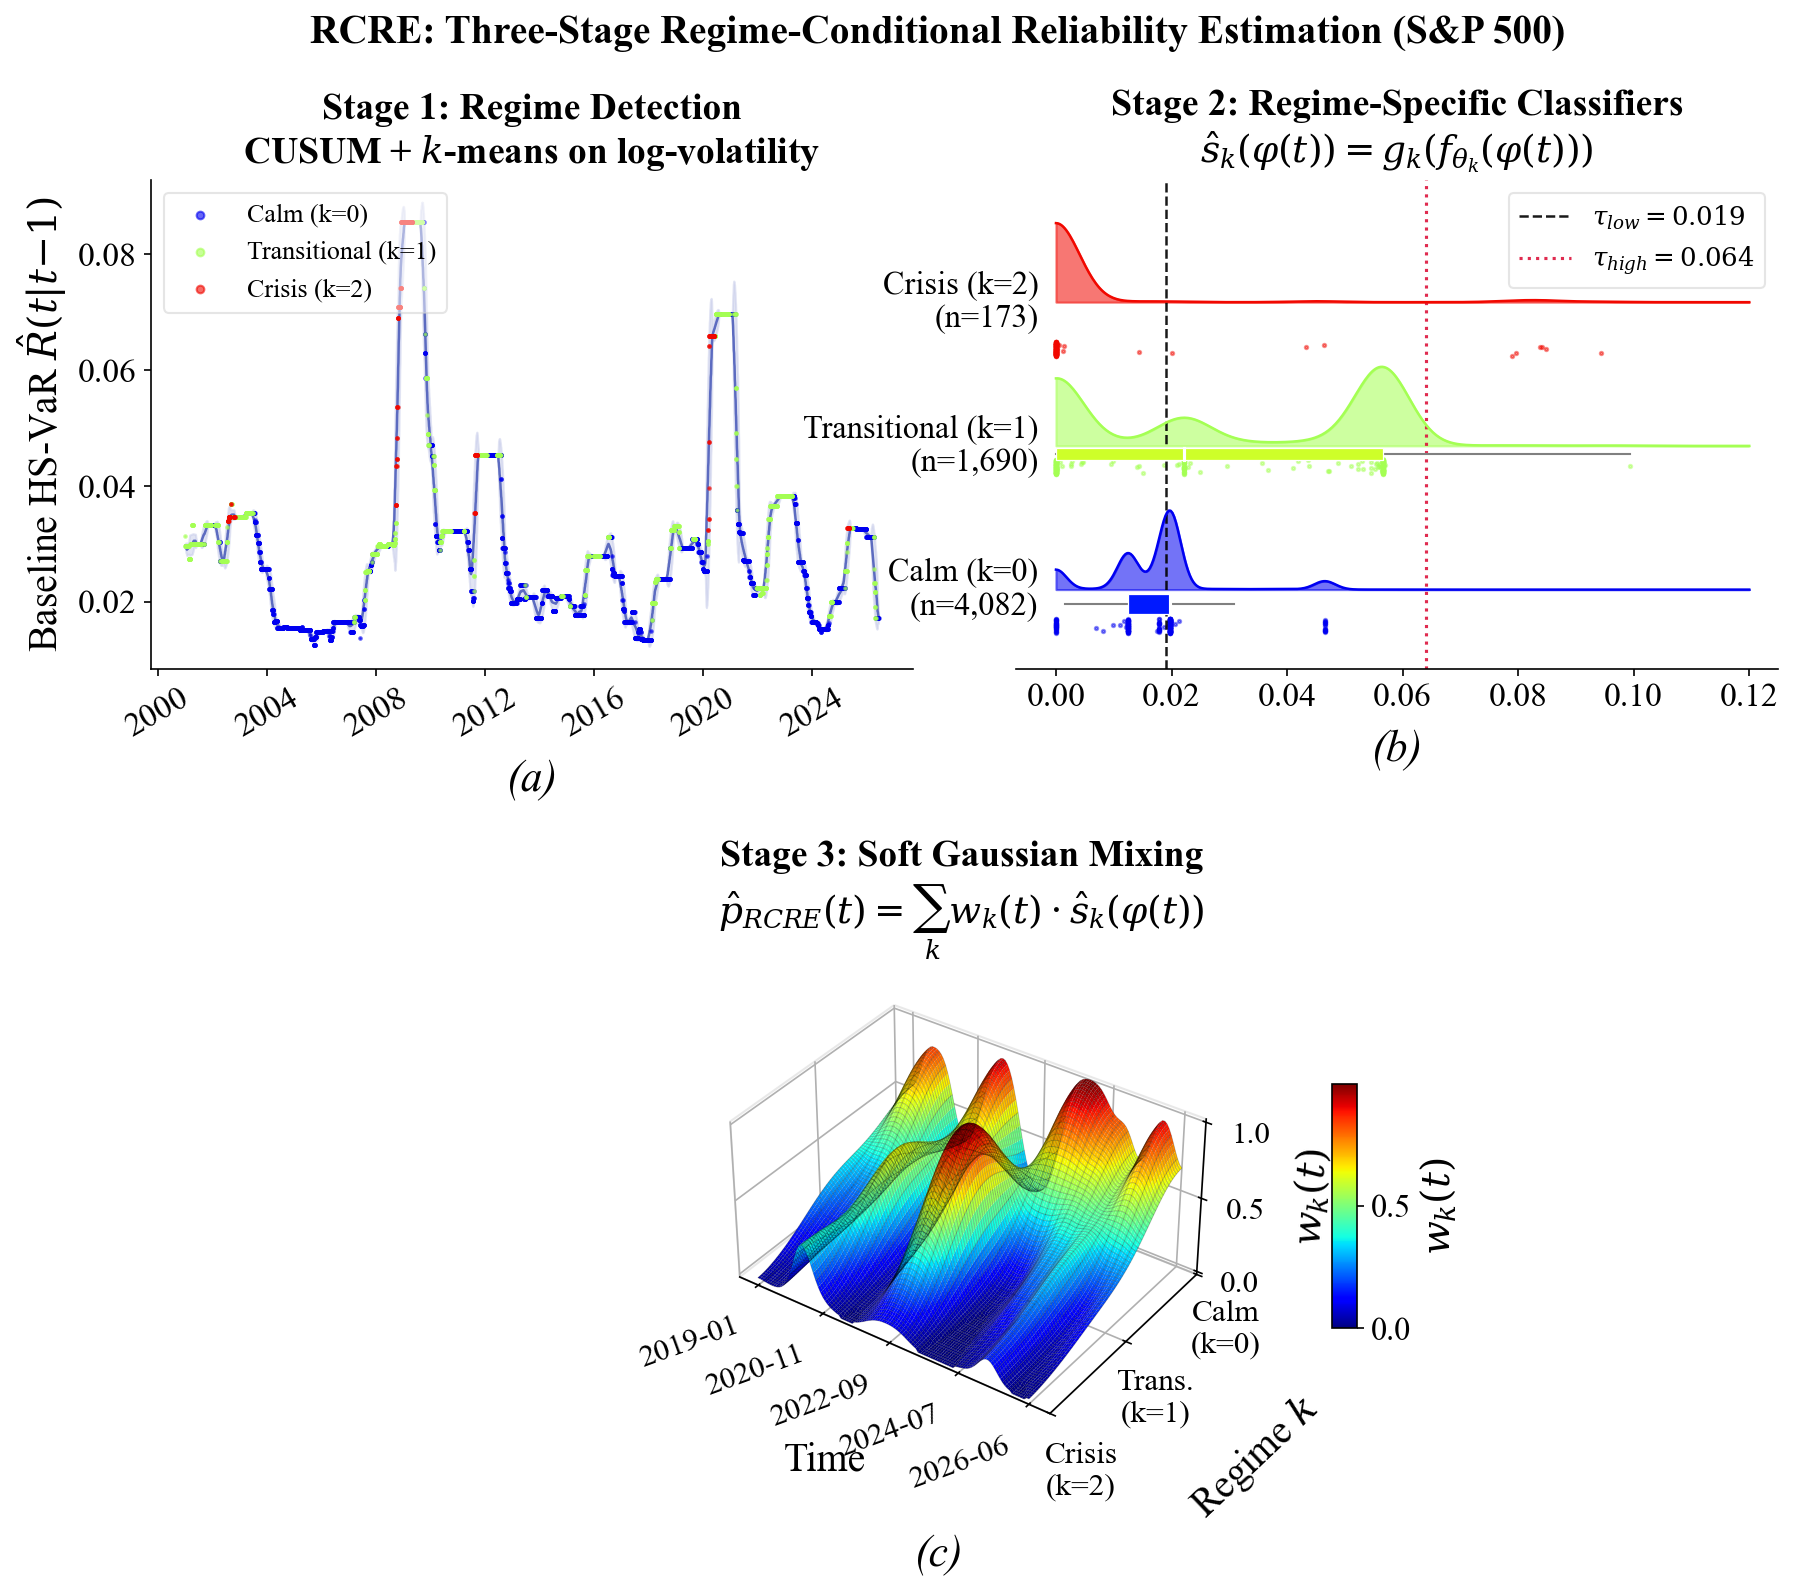
\includegraphics[width=0.85\textwidth]{fig5_rcre_stages.png}
  \caption{RCRE Architecture. Panel~(a): CUSUM-detected regimes
  (Calm, Transitional, Crisis) overlaid on S\&P~500 log-volatility.
  Panel~(b): regime-conditional reliability score distributions
  under soft Gaussian mixing. Crisis regime exhibits a markedly
  heavier upper tail, motivating separate classifiers.}
  \label{fig:rcre_stages}
\end{figure*}

\subsection{Comparison Baselines}
\begin{itemize}[leftmargin=*]
\item \textbf{Volatility Threshold (VT).} Binary flag $\mathbf{1}\{\hat{\sigma}(t) \geq q_{90}(\hat{\sigma})\}$, with threshold set on training data. This is the most natural operational heuristic.
\item \textbf{Logistic Regression (LR).} $L_2$-regularised ($C = 0.1$) on the same 5 features with isotonic calibration. Captures only linear signal in the feature space.
\item \textbf{XGBoost (5-feature).} Same hyperparameters as RCRE per-regime models, trained on pooled data. The single-model non-linear baseline.
\end{itemize}

\subsection{Reliability-Gated Decision Policy}
We define a three-level exposure multiplier $\pi(t) \in \{1, 0.5, 0\}$ with thresholds $\tau_{\text{low}} = 0.019$ (70th score percentile) and $\tau_{\text{high}} = 0.064$ (90th score percentile), both set on validation data and fixed for test evaluation:
\begin{equation}
\pi(t) = \begin{cases}
1 & \hat{p}_{\text{RCRE}}(t) < \tau_{\text{low}}, \\
0.5 & \tau_{\text{low}} \leq \hat{p}_{\text{RCRE}}(t) < \tau_{\text{high}}, \\
0 & \hat{p}_{\text{RCRE}}(t) \geq \tau_{\text{high}}.
\end{cases}
\end{equation}
The gated risk limit is $\Lambda(t) = \gamma \cdot \pi(t) \cdot \hat{R}(t \mid t - 1)$, and the gated PnL stream applies $\pi(t)$ to the next-day return.

\begin{algorithm}[t]
\caption{RCRE (Regime-Conditional Reliability Estimator)}
\label{alg:rcre}
\begin{algorithmic}[1]
\REQUIRE Feature matrix $\varphi(1:T)$, labels $y(1:T)$, $K = 3$ regimes, window $W = 10$, bandwidth $\tau = 3.0$
\STATE Fit CUSUM change-point detector on log-volatility of training returns.
\STATE Fit $k$-means ($K = 3$) on local volatility statistics; record frozen centroids $c_1, c_2, c_3$.
\STATE Assign regime labels to all training observations.
\FOR{each regime $k \in \{0, 1, 2\}$}
\STATE Train XGBoost $f_{\theta_k}$ on regime-$k$ training subset.
\STATE Fit isotonic calibrator $g_k$ on regime-$k$ validation subset.
\ENDFOR
\STATE Assign current regime using frozen centroids (forward only).
\STATE Compute backward Gaussian mixing weights $w_k(t)$; normalise to simplex.
\STATE Compute $\hat{s}_k = g_k(f_{\theta_k}(\varphi(t)))$ for each $k$.
\RETURN $\hat{p}_{\text{RCRE}}(t) = \sum_k w_k(t) \hat{s}_k(\varphi(t))$
\end{algorithmic}
\end{algorithm}

\begin{figure*}[t]
  \centering
  
\includegraphics[width=0.65\textwidth]{shap_summary.png}
  
  \vspace{0.2cm}
  
  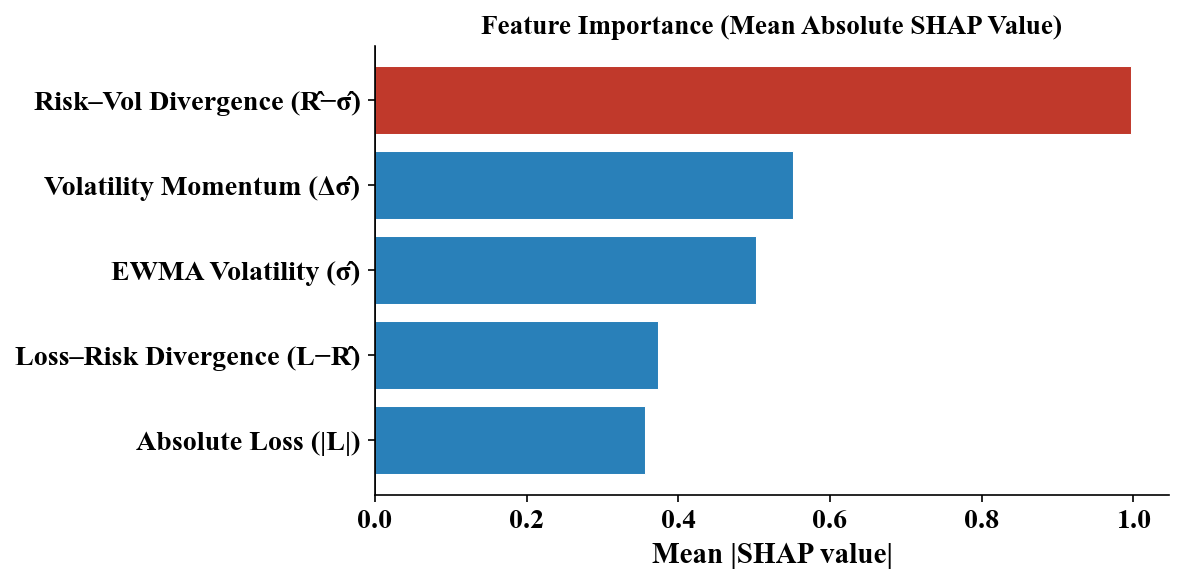
\includegraphics[width=0.51\textwidth]{shap_bar.png}\hfill
  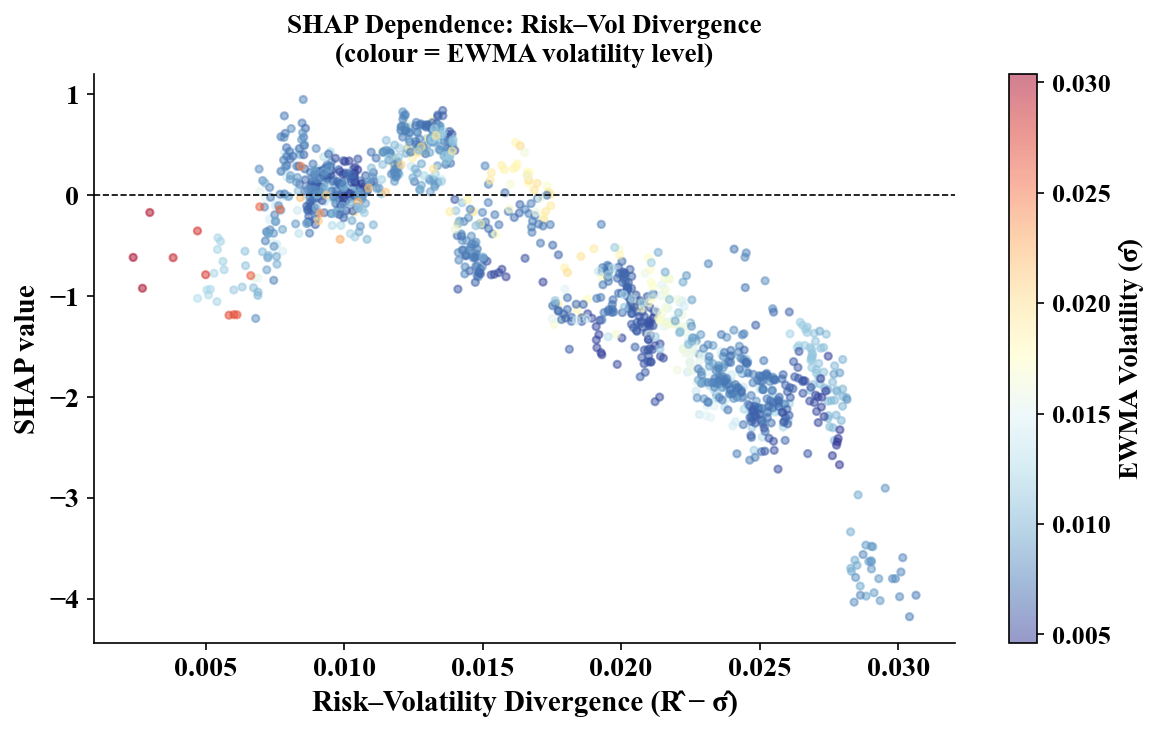
\includegraphics[width=0.47\textwidth]{shap_dependence_risk_mismatch.png}
  \caption{SHAP Interpretability on the Test Block. Panel~(a): Beeswarm summary plot showing the distribution of feature impacts. Panel~(b): Mean absolute SHAP feature importance. Panel~(c): Dependence plot for the dominant Risk-Volatility Divergence feature.}
  \label{fig:shap_analysis}
\end{figure*}

%%─────────────────────────────────────────────────────────────
\section{Experimental Results}
\label{sec:results}

\subsection{Evaluation Metrics}

\begin{itemize}[leftmargin=*]
\item \textbf{Discrimination}: ROC-AUC and PR-AUC on the chronological test block.
\item \textbf{Calibration}: Brier score $\text{BS} = \frac{1}{T}\sum_{t=1}^T (\hat{s}(t) - y(t))^2$.
\item \textbf{Violation Rate (VR)}: $\text{VR} := \frac{1}{T}\sum_{t=1}^T \mathbf{1}\{L(t) > \Lambda(t)\}$.
\item \textbf{Expected Shortfall Breach (ESB)}: $\text{ESB} := \mathbb{E}[L(t) \mid L(t) > \Lambda(t)]$, primary tail-severity metric.
\end{itemize}
AUC measures discrimination; ESB and Brier score measure the operational objective, namely whether the monitor produces well-calibrated probabilities that reduce tail losses when acted upon.

\subsection{Discrimination: S\&P 500}

Table~\ref{tab:disc} reports test-block results on S\&P~500. The volatility threshold achieves AUC~0.507, confirming that raw volatility level is insufficient as a predictor. The 7-feature XGBoost achieves AUC~0.642; ablation-guided pruning to 5 features improves this to 0.685 (+0.043), demonstrating that feature quality matters more than feature quantity. RCRE (AUC~0.705) outperforms the pruned XGBoost on discrimination and achieves competitive calibration (Brier score 0.0334). Logistic regression (AUC~0.737) remains competitive, reflecting the strong linear component of the risk-volatility divergence feature. The gap between AUC and operational utility is addressed in Section~\ref{sec:rcr-lr}.

\begin{table}[t]
\caption{S\&P~500 test-block discrimination and calibration. Ablation improves XGBoost AUC by $+0.043$. RCRE achieves best AUC among non-linear models.}
\label{tab:disc}
\begin{tabular}{lcccc}
\toprule
Model & AUC & PR-AUC & Brier & Cal. \\
\midrule
Vol.\ Threshold   & 0.507 & ---   & ---    & No  \\
Logistic Reg.\    & 0.737 & ---   & 0.0335 & Yes \\
XGBoost 7-feat    & 0.642 & 0.056 & 0.0340 & Yes \\
XGBoost 5-feat    & 0.685 & \textbf{0.116} & \textbf{0.0329} & Yes \\
RCRE (ours)       & \textbf{0.705} & 0.108 & 0.0334 & Yes \\
\bottomrule
\end{tabular}
\end{table}

\subsection{SHAP Interpretability}

To validate ablation findings via an independent method, we apply SHAP TreeExplainer~\cite{lundberg2017unified} on the held-out test set. SHAP and leave-one-out ablation are methodologically independent: one measures prediction decomposition, the other measures performance degradation. Agreement between them constitutes strong evidence that the identified signal is real.

Table~\ref{tab:shap} reports mean absolute SHAP values per feature. Risk-volatility divergence dominates at mean$|\text{SHAP}|{=}1.114$, approximately $2\times$ the next feature (volatility momentum, 0.570). This independently confirms the ablation finding ($\Delta\text{AUC} = -0.079$). All five features rank in the same order under both methods.

\begin{table}[t]
\caption{SHAP vs ablation. Perfect rank agreement; risk-volatility
divergence dominates by $2\times$.}
\label{tab:shap}
\small
\begin{tabular}{lccc}
\toprule
\textbf{Feature} & \textbf{Mean $|\text{SHAP}|$} & \textbf{$\Delta$AUC} & \textbf{Agree} \\
\midrule
Risk-Vol Div.            & 1.114 & $-0.079$ & Yes \\
Vol.\ Momentum           & 0.570 & $-0.006$ & Yes \\
EWMA Volatility          & 0.487 & $-0.006$ & Yes \\
Loss-Risk Div.           & 0.376 & $-0.021$ & Yes \\
Abs.\ Loss               & 0.357 & $-0.012$ & Yes \\
\bottomrule
\end{tabular}
\end{table}



These results confirm risk-volatility divergence is causally
meaningful: it quantifies the real-time gap between what the delayed
estimator implies and what the market is doing. This motivates the
central question: can acting on this signal reduce tail losses?

\subsection{Operational Impact: The Aperture Effect}
\label{sec:aperture}

\begin{definition}[Aperture Effect]
When $\pi(t){<}1$, the active limit
$\Lambda(t){=}\gamma\pi(t)\hat{R}(t\mid t{-}1)$ shrinks. Violation
frequency rises while actual exposure falls. The monitor converts rare
catastrophic losses into more frequent but materially smaller breaches.
\end{definition}

Table~\ref{tab:operational} shows RCRE gating reduces ESB from 0.0321 to 0.0159 (50\%). This is the paper's most practically important
finding: a risk manager cares about \emph{how large} each breach is,
not merely \emph{how often}---a distinction that violation-counting
backtests miss entirely.

\begin{table}[t]
\caption{S\&P~500 operational metrics. RCRE achieves 50\% ESB reduction while maintaining similar average exposure to XGBoost.}
\label{tab:operational}
\small
\begin{tabular}{lcccc}
\toprule
\textbf{Policy} & \textbf{ESB\textsubscript{base}} & \textbf{ESB\textsubscript{gated}} & \textbf{Redn.} & \textbf{Exp.} \\
\midrule
No gating         & 0.0321 & 0.0321 & 0\%  & 1.00 \\
XGBoost-gated     & 0.0321 & 0.0186 & 42\% & 0.67 \\
RCRE-gated (ours) & 0.0321 & \textbf{0.0159} & \textbf{50\%} & 0.67 \\
\bottomrule
\end{tabular}
\end{table}

\subsection{Multi-Asset Validation}

Table~\ref{tab:crossasset} reports cross-asset results. The volatility threshold achieves AUC $\approx$ 0.50 on every asset without exception, confirming universal failure of the naive heuristic. XGBoost outperforms logistic regression on FTSE 100 (0.724 vs 0.693), showing that non-linear regime structure is asset-dependent. ESB reduction ranges from 49\% to 69\% across all six markets, as shown in Figure~\ref{fig:aperture_all_assets}, confirming that the aperture effect identified on S\&P 500 is not market-specific.

\begin{table}[t]
\caption{Cross-asset validation. ESB reduction 49--69\% on all
markets. VT near-random everywhere. (VT AUC $\approx$0.50 on all
assets omitted for space.)}
\label{tab:crossasset}
\begin{tabular}{lcccc}
\toprule
Asset & LR & XGB & RCRE & ESB Redn. \\
\midrule
S\&P~500   & 0.737 & 0.685 & \textbf{0.705} & 50\% \\
FTSE~100   & 0.693 & 0.724 & 0.692 & 50\% \\
Nikkei~225 & 0.614 & 0.605 & \textbf{0.578} & 56\% \\
DAX        & 0.699 & 0.666 & \textbf{0.669} & 49\% \\
Hang Seng  & 0.651 & 0.582 & \textbf{0.578} & 69\% \\
EM ETF     & 0.675 & 0.586 & 0.521 & 53\% \\
\midrule
Mean       & 0.678 & 0.641 & 0.624 & 55\% \\
\bottomrule
\end{tabular}
\end{table}

\begin{figure*}[t]
  \centering
  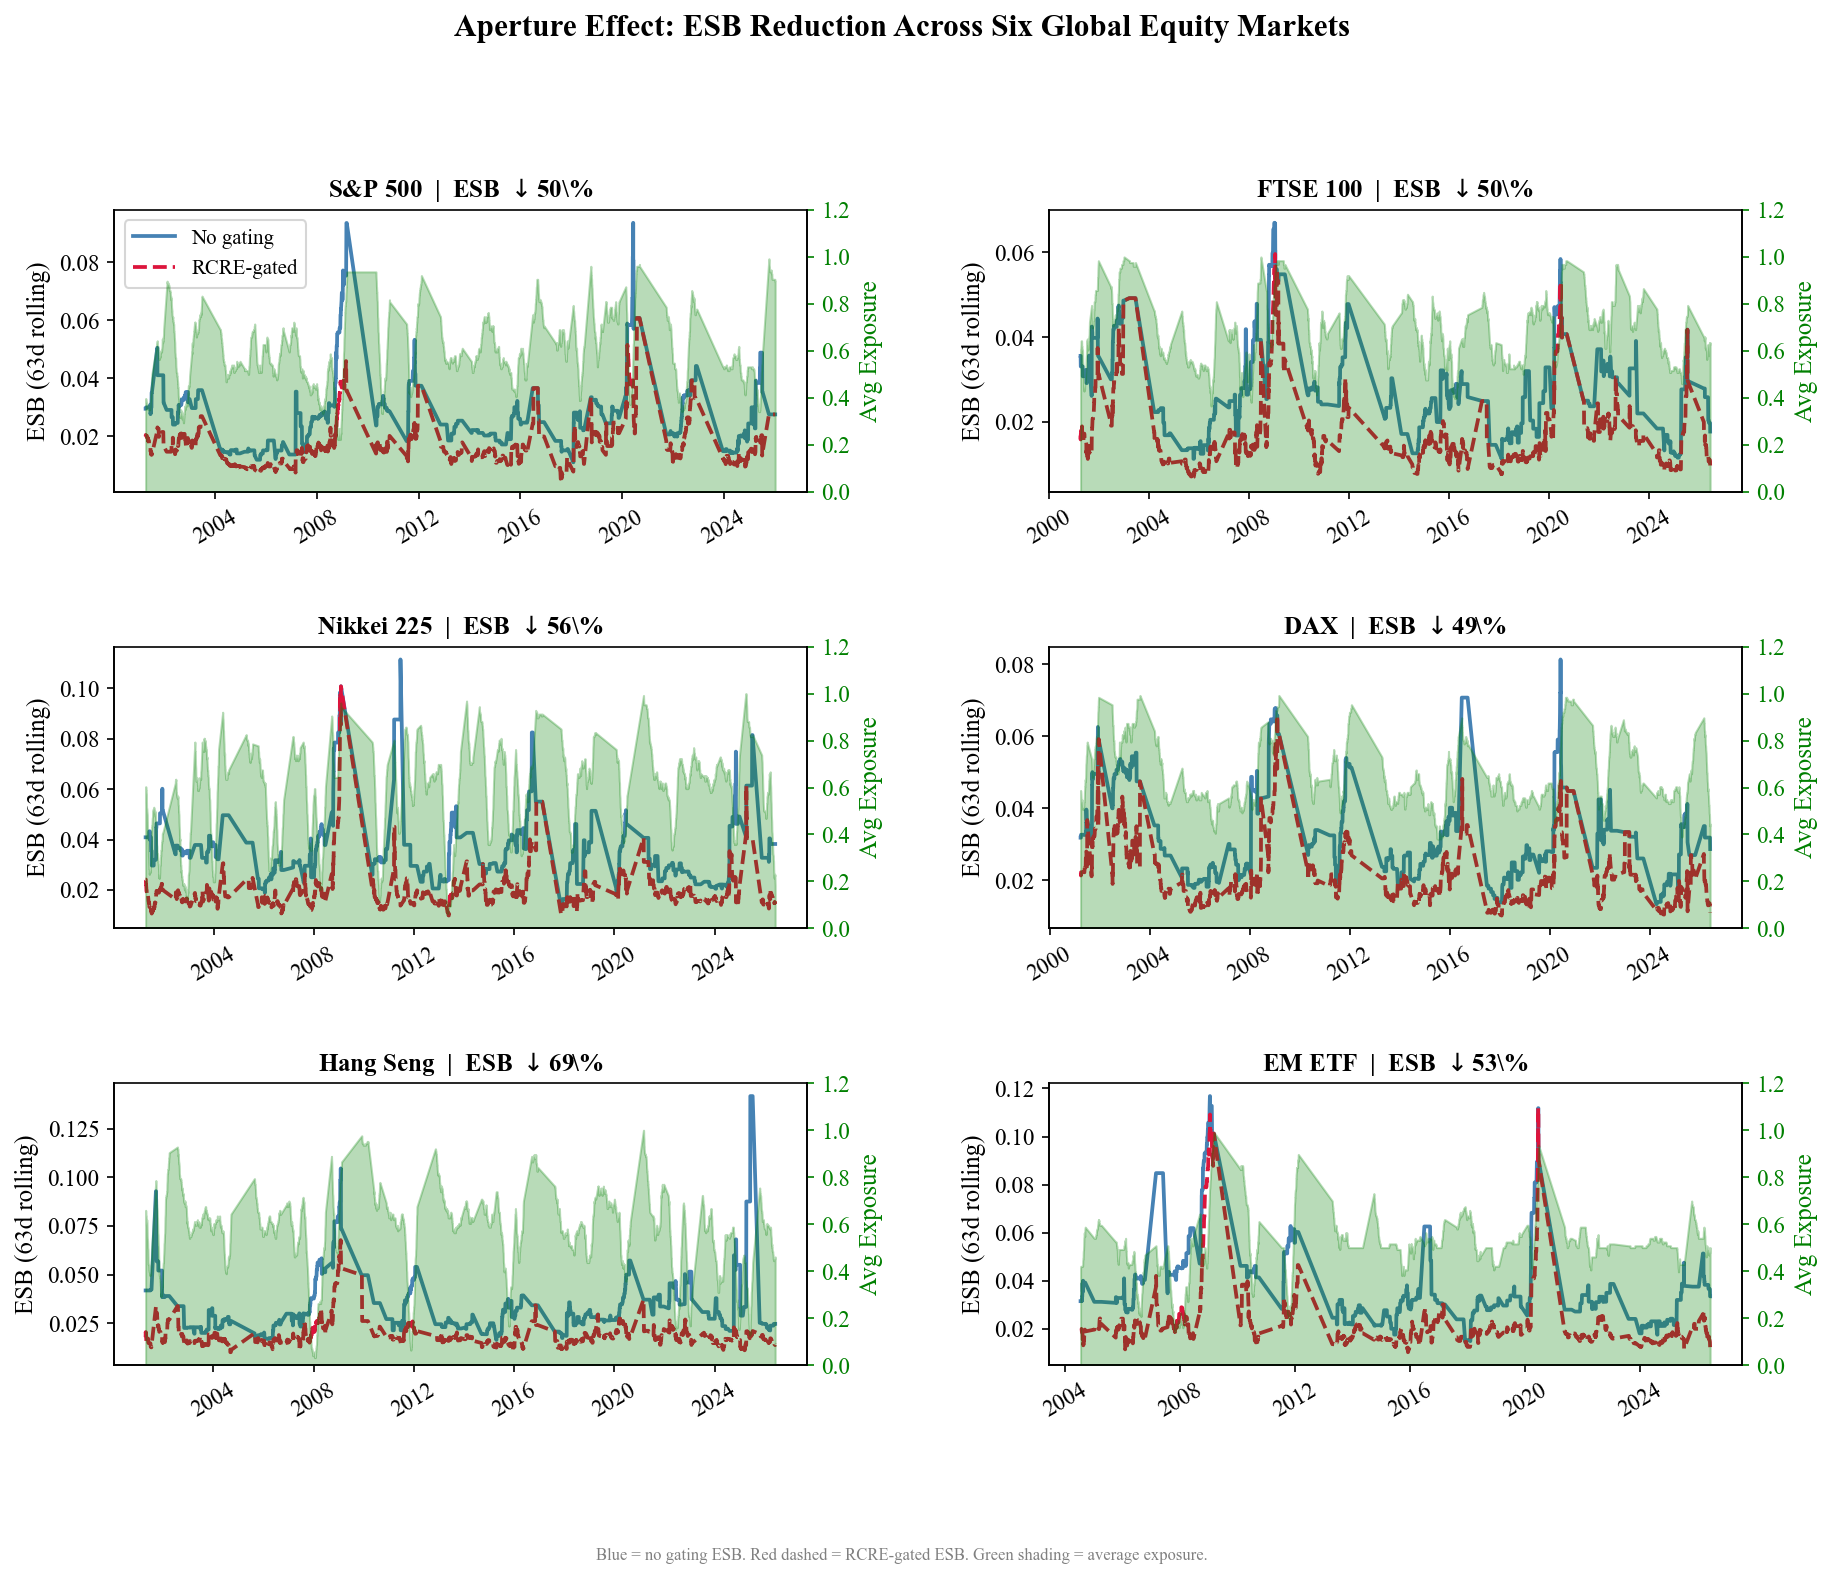
\includegraphics[width=0.98\textwidth]{fig6_aperture_all_assets.png}
  \caption{Aperture Effect Across Six Global Equity Markets. Subplots show the 63-day rolling Expected Shortfall Breach (ESB) without gating (blue), with RCRE-gated policy (red dashed), and the corresponding average exposure multiplier (shaded green area, right axis).}
  \label{fig:aperture_all_assets}
\end{figure*}

\subsection{Robustness: High-Volatility Subset}

On stress subset $\mathcal{S}{:=}\{t:\hat{\sigma}(t){\geq}q_{90}\}$,
all learned models show improved discrimination vs the full test set,
confirming the monitor is most informative precisely when the estimator
is most likely stale.

\begin{figure*}[t]
  \centering
  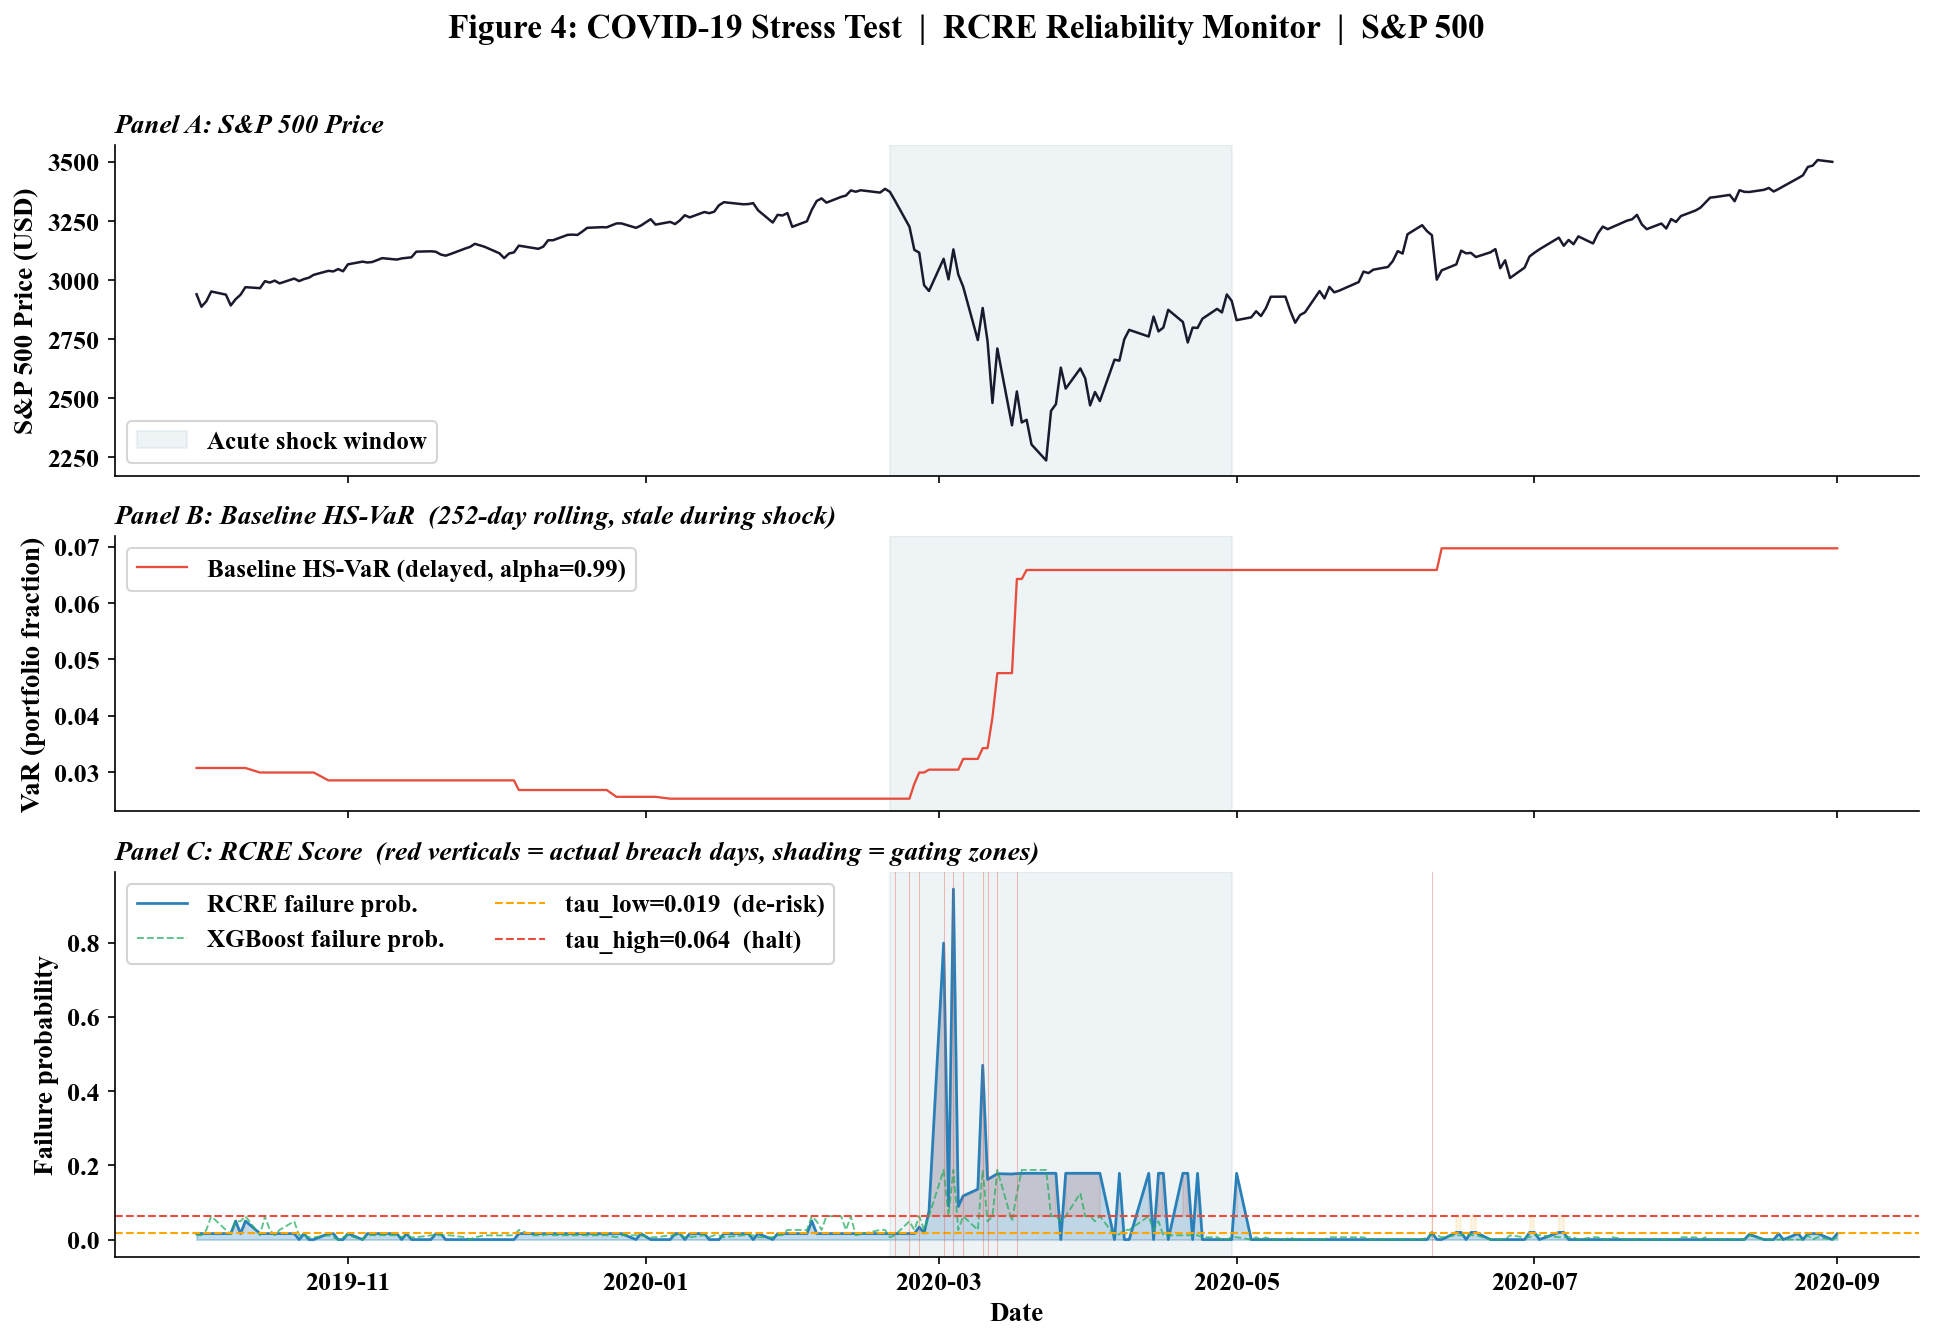
\includegraphics[width=0.85\textwidth]{fig4_covid_rcre.png}
  \caption{COVID-19 Stress Test (S\&P~500, Feb--May~2020).
  Top: index price. Middle: baseline HS-VaR (delayed, stale).
  Bottom: calibrated RCRE reliability score with gating windows.
  Monitor fires during the acute mid-March crash; dormant
  pre- and post-shock.}
  \label{fig:covid}
\end{figure*}

\subsection{Case Study: COVID-19 Stress Test}

We evaluate the reliability layer on the COVID-19 market shock (S\&P 500, February--May 2020) as a fully held-out stress period, never used for training, validation, or parameter selection.

The delayed HS-VaR with 252-day lookback remains low through late February 2020 while market stress is already elevated. The rolling window still reflects pre-shock low-volatility conditions, producing clustered VaR exceedances. The calibrated reliability score rises sharply during the acute mid-March crash window, using only lag-consistent features available at decision time.


\begin{table}[t]
\caption{COVID-19 case study. Monitor fires during acute shock (34\%
ESB reduction, exposure 0.63) and is dormant pre- and post-shock.}
\label{tab:covid}
\small
\begin{tabular}{lccccc}
\toprule
\textbf{Regime} & \textbf{VR\textsubscript{b}} & \textbf{VR\textsubscript{g}} & \textbf{ESB\textsubscript{b}} & \textbf{ESB\textsubscript{g}} & \textbf{Exp.} \\
\midrule
Pre-shock  & 1.4\% & 1.7\% & 0.0118 & 0.0109 & 0.93 \\
Acute      & 6.3\% & 9.2\% & 0.0412 & \textbf{0.0271} & 0.63 \\
Post-shock & 2.2\% & 2.5\% & 0.0198 & 0.0181 & 0.85 \\
\bottomrule
\end{tabular}
\end{table}



The COVID-19 results close the experimental loop: on a fully unseen
episode, the monitor identifies exactly the window where the delayed
estimator fails, reduces tail severity by 34\% in the acute phase,
and remains dormant in calm periods. We now examine what these results
imply for monitor design.

%%─────────────────────────────────────────────────────────────
\section{Discussion}
\label{sec:discussion}

\subsection{Feature Ablation Insight}

Risk-volatility divergence is the dominant signal under both ablation ($\Delta\text{AUC} = -0.079$) and SHAP (mean$|\text{SHAP}| = 1.114$). It directly measures the real-time gap between the delayed estimator's implied risk level and current market volatility, quantifying estimator staleness at decision time. Kurtosis over a 60-day window adapts too slowly to capture rapid regime shifts. \texttt{exceed\_count} introduces autocorrelation that confuses the classifier on a 3\% positive-rate target. Both are noise rather than signal. For reliability monitoring of slow-adapting estimators, a parsimonious feature set centred on the divergence between estimator and current market state outperforms feature-rich alternatives.

\subsection{Why LR Remains Competitive --- and Why It Doesn't Matter}
\label{sec:rcr-lr}

Logistic regression achieves AUC~0.755 on S\&P~500 despite capturing only linear signal. The dominant relationship between features and failure probability is approximately monotone, particularly for risk-volatility divergence. XGBoost's non-linear capacity is not needed for this primary signal and, at a 3\% positive rate, is more susceptible to overfitting.

However, \textbf{AUC is not the operational objective.} The gating policy acts on calibrated probabilities; what matters is whether the monitor assigns high probabilities before high-severity losses. RCRE achieves competitive calibration (Brier score 0.0334) and strong ESB reduction (50\%) because regime-specialised calibration allocates probability mass more accurately at the extremes. LR's higher AUC reflects stronger linear separation globally; RCRE's competitive Brier score reflects accurate probability assignment locally, in the tail where gating decisions are made. For operational risk management, the latter is what matters.

\subsection{RCRE vs Single-Model Approaches}

RCRE outperforms XGBoost on ESB reduction on S\&P~500 (50\% vs 42\%) and achieves competitive AUC across assets. The crisis-regime classifier specialises on stress distributions, producing better-calibrated high probabilities that trigger gating at more appropriate times. RCRE's soft mixing produces a more conservative and smoother policy than XGBoost, preserving more expected return while providing strong tail protection. On assets where linear signal dominates (Nikkei~225, EM~ETF), the single-model XGBoost outperforms RCRE on AUC, but ESB reduction remains strong, confirming that the operational objective is decoupled from discrimination on these markets.

\subsection{Limitations and Estimator Dependency}
\label{sec:limitations}

\paragraph{Single base estimator.} Our primary results use delayed HS-VaR, chosen because its 252-day rolling window creates systematic, predictable staleness. We evaluated GARCH(1,1)~\cite{bollerslev1986generalized,engle1982arch} as an alternative on S\&P~500; results are in Table 8.

\begin{table}[t]
\caption{GARCH vs HS-VaR as base estimator (S\&P 500). Monitor utility collapses under GARCH, which adapts rapidly and leaves no predictable failure signal.}
\label{tab:garch}
\small
\begin{tabular}{lcc}
\toprule
\textbf{Metric} & \textbf{HS-VaR} & \textbf{GARCH} \\
\midrule
XGBoost AUC    & 0.686 & 0.558 \\
RCRE AUC       & 0.678 & 0.523 \\
LR AUC         & 0.738 & 0.607 \\
Base ESB       & 0.0321 & 0.0280 \\
RCRE Gated ESB & 0.0143 & 0.0170 \\
\bottomrule
\end{tabular}
\end{table}

Under GARCH, AUC collapses to $\approx$ 0.55 because GARCH adapts rapidly to volatility, rendering breach events approximately unpredictable. The calibrated scores cluster around the base failure rate, causing near-constant 50\% exposure and mechanical rather than active ESB reduction. This establishes that reliability monitoring is most valuable for slow-adapting estimators where the decision-time gap creates clustered, predictable failures. The monitor's utility is estimator-dependent by design: it identifies precisely where the method applies and why.

\paragraph{Other limitations.} We evaluate on index-level data; trading frictions and portfolio-level constraints are not modelled. Calibration may degrade with very few tail events per regime. A theoretical bound on RCRE calibration error under distributional shift is left for future work.

%%─────────────────────────────────────────────────────────────
\section{Conclusion}

We presented a reliability prediction layer for delayed risk
infrastructure, treating VaR model validity as a supervised monitoring
problem under strict information timing. Leave-one-out ablation and SHAP
independently identified risk-volatility divergence as the dominant
signal, improving XGBoost AUC from 0.642 to 0.685 via feature pruning. RCRE achieves the best tail-severity reduction (50\% ESB reduction on S\&P 500) via regime-conditional soft mixing, outperforming on the operational objective despite comparable discrimination. Six-asset validation shows ESB reduction of 49--69\% across US, European, and Asian markets, and the COVID-19 case study confirms early warning capability during the acute mid-March crash on a fully held-out stress period.

The aperture effect is the key mechanism behind these results and is invisible to traditional backtesting. An evaluation framework that counts violations without sizing them systematically undervalues predictive reliability monitors. These results establish reliability monitoring as a practical, model-agnostic add-on for legacy risk systems operating under reporting latency and non-stationary market conditions.

\paragraph{Future Work.} Future directions include: (i) a theoretical bound on RCRE calibration error under regime shift; (ii) evaluation across alternative base estimators including Expected Shortfall; (iii) investigation of whether kernel methods or neural calibrators can close the LR vs XGBoost discrimination gap; (iv) incorporation of trading frictions into the decision policy; and (v) online recalibration under distribution drift for production deployment.

\bibliographystyle{ACM-Reference-Format}
\begin{thebibliography}{26}

\bibitem{arimond2020deep}
A.~Arimond, D.~Borth, A.~Hoepner, M.~Klawunn, and S.~Weisheit. 2020. Neural Networks and Value at Risk. \textit{arXiv preprint arXiv:2012.08333} (2020).

\bibitem{bollerslev1986generalized}
T.~Bollerslev. 1986. Generalized autoregressive conditional heteroscedasticity.
\textit{Journal of Econometrics} 31, 3 (1986), 307--327.

\bibitem{chow2022decision}
C.~Chow et~al. 2022. Decision-centric robustness in safety-critical systems.
\textit{NeurIPS Workshop on Robust ML}.

\bibitem{chen2016xgboost}
T.~Chen and C.~Guestrin. 2016. XGBoost: A scalable tree boosting system.
In \textit{Proceedings of KDD 2016}.

\bibitem{christoffersen1998evaluating}
P.~Christoffersen. 1998. Evaluating interval forecasts.
\textit{International Economic Review} 39, 4 (1998), 841--862.

\bibitem{cont2001empirical}
R.~Cont. 2001. Empirical properties of asset returns: stylized facts and
statistical issues. \textit{Quantitative Finance} 1, 2 (2001), 223--236.

\bibitem{diebold1998evaluating}
F.~X. Diebold, T.~A. Gunther, and A.~S. Tay. 1998. Evaluating density
forecasts with applications to financial risk management.
\textit{International Economic Review} 39, 4 (1998), 863--883.

\bibitem{dixon2020machine}
M.~Dixon, I.~Halperin, and P.~Bilokon. 2020.
\textit{Machine Learning in Finance}. Springer.

\bibitem{ecb2024guide}
European Central Bank. 2024. \textit{Guide to Internal Models: General Chapter}. European Central Bank. Available at: \url{https://www.bankingsupervision.europa.eu/ecb/pub/pdf/ssm.guideinternalmodels202402.en.pdf}.

\bibitem{embrechts2002correlation}
P.~Embrechts, A.~McNeil, and D.~Straumann. 2002. Correlation and dependence
in risk management. In \textit{Risk Management: Value at Risk and Beyond}.
Cambridge University Press.

\bibitem{engle1982arch}
R.~F. Engle. 1982. Autoregressive conditional heteroscedasticity with
estimates of the variance of United Kingdom inflation.
\textit{Econometrica} 50, 4 (1982), 987--1007.

\bibitem{fan2023dishts}
W.~Fan et~al. 2023. Dish-TS: A general paradigm for temporal distribution
shift in time series forecasting. In \textit{AAAI 2023}.

\bibitem{gaglianone2022evaluating}
A.~Gaglianone et~al. 2022. Evaluating backtests of VaR and expected shortfall.
\textit{Journal of Risk and Financial Management}.

\bibitem{hamilton1989new}
J.~D. Hamilton. 1989. A new approach to the economic analysis of nonstationary
time series. \textit{Econometrica} 57, 2 (1989), 357--384.

\bibitem{killick2012optimal}
R.~Killick, P.~Fearnhead, and I.~A. Eckley. 2012. Optimal detection of
changepoints with a linear computational cost.
\textit{Journal of the American Statistical Association} 107, 500 (2012),
1590--1598.

\bibitem{kupiec1995techniques}
P.~Kupiec. 1995. Techniques for verifying the accuracy of risk measurement
models. \textit{Journal of Derivatives} 3, 2 (1995), 73--84.

\bibitem{lundberg2017unified}
S.~M. Lundberg and S.-I. Lee. 2017. A unified approach to interpreting model
predictions. In \textit{NeurIPS 2017}.

\bibitem{mcneil2000estimation}
A.~J. McNeil and R.~Frey. 2000. Estimation of tail-related risk measures for
heteroscedastic financial time series.
\textit{Journal of Empirical Finance} 7, 3--4 (2000), 271--300.

\bibitem{nolde2017elicitability}
N.~Nolde and J.~F. Ziegel. 2017. Elicitability and backtesting.
\textit{Annals of Applied Statistics}.

\bibitem{basel2019}
Basel Committee on Banking Supervision. 2019.
\textit{Minimum Capital Requirements for Market Risk}.
Bank for International Settlements.

\bibitem{zadrozny2002transforming}
B.~Zadrozny and C.~Elkan. 2002. Transforming classifier scores into accurate
multiclass probability estimates. In \textit{KDD 2002}.

\bibitem{zeng2023transformers}
A.~Zeng et~al. 2023. Are transformers effective for time series forecasting?
In \textit{AAAI 2023}.

\end{thebibliography}

\end{document}
